% Szglab4
% ===========================================================================
%
\chapter{Szkeleton tervezése}

\thispagestyle{fancy}

\section{A szkeleton modell valóságos use-case-ei}
\comment{A szkeletonnak, mint önálló programnak a működésével kapcsolatos use-case-ek.}

\subsection{Use-case diagram}

\begin{figure}[h]
\begin{center}
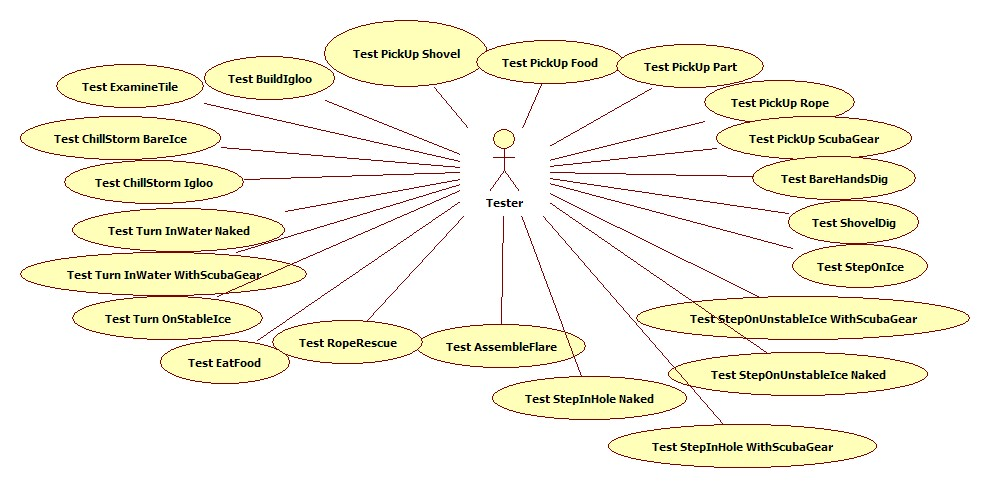
\includegraphics[width=17cm]{chapters/chapter05/diagrams/TesztUseCase.jpg}
\caption{Use-case}
\label{fig:SzkeletonUseCase}
\end{center}
\end{figure}

\subsection{Use-case leírások}
% TODO: Valaki latexhez értő írja ezeket át itemize-ra, mert a latex jobbra húzza a bekezdés első sorát.
\usecase{Test PickUp Shovel}{Játékos lapátot vesz fel.}{Tester}{
	1. Eszkimó hóval nem rendelkező jégtáblán áll, amin egy lapát található.\newline
	2. Az eszkimó energiája csökken.\newline
	2.A Az eszkimó fáradt és nem tud tárgyat felvenni.\newline
	3. Az eszkimó felveszi a lapátot.\newline
	4. A lapát bekerül az eszkimó tárgyai közé és a megfelelő stratégiája helyére is.
}
\usecase{Test PickUp Food}{Játékos ételt vesz fel.}{Tester}{
	1. Eszkimó hóval nem rendelkező jégtáblán áll, amin egy élelem található.\newline
	2. Az eszkimó energiája csökken.\newline
	2.A Az eszkimó fáradt és nem tud tárgyat felvenni.\newline
	3. Az eszkimó felveszi az élelmet
	4. Az élelem bekerül az eszkimó tárgyai közé és a kajatárolójába is.
}
\usecase{Test PickUp Part}{Játékos alkatrészt vesz fel.}{Tester}{
	1. Eszkimó hóval nem rendelkező jégtáblán áll, amin egy rakéta alkatrész található.\newline
	2. Az eszkimó energiája csökken.\newline
	2.A Az eszkimó fáradt és nem tud tárgyat felvenni.\newline
	3. Az eszkimó felveszi az alkatrészt.\newline
	4. Az alkatrész bekerül az eszkimó tárgyai közé és a rakétadarabtárolójába is.
}
\usecase{Test PickUp Rope}{Játékos kötelet vesz fel.}{Tester}{
	1. Eszkimó hóval nem rendelkező jégtáblán áll, amin egy kötél található.\newline
	2. Az eszkimó energiája csökken.\newline
	2.A Az eszkimó fáradt és nem tud tárgyat felvenni.\newline
	3. Az eszkimó felveszi a kötelet.\newline
	4. A kötél bekerül az eszkimó tárgyai közé és a megfelelő stratégiája helyére is.
}
\usecase{Test PickUp ScubaGear}{Játékos búváruhát vesz fel.}{Tester}{
	1. Eszkimó hóval nem rendelkező jégtáblán áll, amin egy búvárruha található.\newline
	2. Az eszkimó energiája csökken.\newline
	2.A Az eszkimó fáradt és nem tud tárgyat felvenni.\newline
	3. Az eszkimó felveszi a búvárruhát.\newline
	4. A búvárruha bekerül az eszkimó tárgyai közé és a megfelelő stratégiája helyére is.
}
\usecase{Test BareHandsDig}{Játékos üres kézzel havat lapátol.}{Tester}{
	1. Eszkimó hóval rendelkező jégtáblán áll.\newline
	2. Az eszkimó energiája csökken.\newline
	2.A Az eszkimó fáradt és nem tud tárgyat felvenni.\newline
	3. Az eszkimó a lapátja segítségével 2 havat ellapátol a jégtábláról.
} 
\usecase{Test ShovelDig}{Játékos lapáttal havat lapátol.}{Tester}{
	1. Eszkimó hóval rendelkező jégtáblán áll.\newline
	2. Az eszkimó energiája csökken.\newline
	2.A Az eszkimó fáradt és nem tud tárgyat felvenni.\newline
	3. Az eszkimó a keze segítségével 1 havat ellapátol a jégtábláról.
} 
\usecase{Test StepOnIce}{Játékos jégre lép.}{Tester}{
	1. Eszkimó jégtáblán áll és van előtte egy másik jégtábla.\newline
	2. Az eszkimó energiája csökken.\newline
	2.A Az eszkimó fáradt és nem tud előrelépni.\newline
	3. Az eszkimó előrelép.
}
\usecase{Test StepOnUnstableIce WithScubaGear}{Búvárruhás játékos instabil jégre lép.}{Tester}{
	1. Búvárruhás eszkimó jégtáblán áll és van előtte egy másik jégtábla, ami csak egy főt bír el, és áll rajta egy másik eszkimó.\newline
	2. Az eszkimó energiája csökken.\newline
	2.A. Alter: Az eszkimó fáradt és nem tud előrelépni.\newline
	3. Az eszkimó előrelép.\newline
	4. A jégtábla beszakad.\newline
	5. A búvárruha megvédi az eszkimót a hideg víztől.
}
\usecase{Test StepOnUnstableIce Naked}{Játékos instabil jégre lép.}{Tester}{
	1. Eszkimó jégtáblán áll és van előtte egy másik jégtábla, ami csak egy főt bír el, és áll rajta egy másik eszkimó.\newline
	2. Az eszkimó energiája csökken.\newline
	2.A Az eszkimó fáradt és nem tud előrelépni.\newline
	3. Az eszkimó előrelép.\newline
	4. A jégtábla beszakad.\newline
	5. Az eszkimó elkezd fuldokolni a hideg vízben.
}
\usecase{Test StepInHole WithScubaGear}{Búvárruhás játékos lyukba esik.}{Tester}{
	1. Búvárruhás eszkimó jégtáblán áll és van előtte egy hóval fedett lyuk.\newline
	2. Az eszkimó energiája csökken.\newline
	2.A Az eszkimó fáradt és nem tud előrelépni.\newline
	3. Az eszkimó előrelép.\newline
	4. A hó beszakad.\newline
	5. A búvárruha megvédi az eszkimót a hideg víztől.
}
\usecase{Test StepInHole Naked}{Játékos lyukba esik.}{Tester}{
	1. Búvárruhás eszkimó jégtáblán áll és van előtte egy hóval fedett lyuk.\newline
	2. Az eszkimó energiája csökken.\newline
	2.A Az eszkimó fáradt és nem tud előrelépni.\newline
	3. Az eszkimó előrelép.\newline
	4. A hó beszakad.\newline
	5. Az eszkimó elkezd fuldokolni a hideg vízben.
}
\usecase{Test RopeRescue}{...}{Tester}{...}
\usecase{Test EatFood}{...}{Tester}{...}
\usecase{Test AssebleFlare}{...}{Tester}{...}
\usecase{Test BuildIgloo}{...}{Tester}{...}
\usecase{Test ExamineTile}{...}{Tester}{...}
\usecase{Test Test Turn OnStableIce}{Játékos elkezdi a körét sima jégen.}{Tester}{
	1. Eszkimó jégtáblán áll, amikor elkezdődik a kör. \newline
	2. Az eszkimó energiája feltöltődik. \newline
}
\usecase{Test Test Turn InWater WithScubaGear}{Játékos elkezdi a körét vízen búvárruhában.}{Tester}{
	1. Eszkimó búvárruhában vízben áll, amikor elkezdődik a kör. \newline
	2. Az eszkimó energiája feltöltődik. \newline
}
\usecase{Test Test Turn InWater Naked}{Játékos elkezdi a körét vízen búvárruha nélkül.}{Tester}{
	1. Eszkimó vízben fulladozik, amikor elkezdődik a kör. \newline
	2. Az eszkimó testhője fogy. \newline
	2.A Az eszkimó teljesen belefagyott a vízbe, nincs több testhője, a játék véget ér.
}
\usecase{Test ChillStorm Igloo }{Játékost igluban éri a hóvihar.}{Tester}{
	1. Eszkimó egy jégtáblán áll, ahol már van iglu. \newline
	2. Jön a hóvihar, de az eszkimót ez nem érdekli, ő nem fázik. \newline
}
\usecase{Test ChillStorm BareIce}{Játékost iglu nélküli jégen éri a hóvihar}{Tester}{
	1. Eszkimó egy jégtáblán áll, ahol nincs iglu. \newline
	2. Jön a hóvihar, és a szegény eszkimó fázik, a testhőjéből veszít. \newline
	2.A Jön a hóvihar, viszont az eszkimó teljesen megfagyott, nincs több testhője, a játék véget ér. \newline
}

\section{A szkeleton kezelői felületének terve, dialógusok}
\comment{A szkeleton által elfogadott bemenetek , valamint a szöveges konzolon megjelenő kimenetek. A kiemenet formátuma olyan kell legyen, ami alapján a működés összevethető a korábbi szekvencia-diagramokkal.}

A szkeleton program működésének ellenőrzéséhez egy saját osztályt fogunk létrehozni. A szkeleton program szöveges formátumban fogja megjeleníteni a függvény hívásokat és visszatérési értéküket, ezzel a szekvenciadiagrammokkal való egyezés majd könnyen ellenőrizhető lesz. Induláskor majd egy menü segítségével lehet választani a különböző szekvenciák közül. A menüt a konzolos ablakban a billentyűzet segítségével lehet majd vezérelni. A menüpontok amiből választani lehet így néz ki:
\begin{Verbatim}[samepage=true]
1. játékos
	1. tárgyat vesz fel
		1. lapát
		2. kötél
		3. alkatrész
		...
	2. havat lapátol
		1. lapáttal
		2. üres kézzel
		...
\end{Verbatim}
A szkeleton programban az objektumok csak asszociációkat tárolnak, egyéb állapotokat a felhasználótól kér majd be. Ezeket szintén a menüvezérelt módszerrel teszi. Kiválasztva egy esetet a teljes szekvencia lefutása automatikus, a kimenet következő képpen néz majd ki a konzolban:
\begin{Verbatim}[samepage=true]
myLoggerTest.DoTest() {
    myLoggerTest.fn1() {
        myDummyObject.DummyObject() {
        }
        myLoggerTest.fn2(myDummyObject, 10) {
            myDummyObject.fn3(20) {
            }
            return 1234;
        }
        return myDummyObject;
    }
}
\end{Verbatim}
A bejegyzésben objektum név . függvénynév (paraméterek) \{ ... \} formátumban jelenek meg a függvényhívások. A visszatérési értéket pedig a return után írja ki.

\pagebreak
\section{Szekvencia diagramok a belső működésre}

\begin{figure}[h]
	\begin{center}
		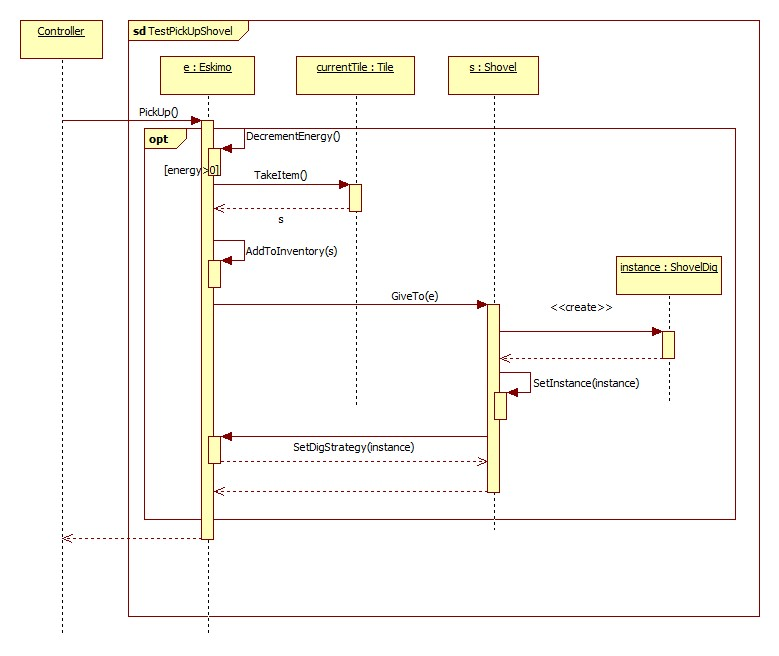
\includegraphics[width=17cm]{chapters/chapter05/diagrams/TestPickUpShovel.jpg}
		\caption{Test PickUp Shovel}
		\label{fig:Test PickUp Shovel}
	\end{center}
\end{figure}

\begin{figure}[h]
	\begin{center}
		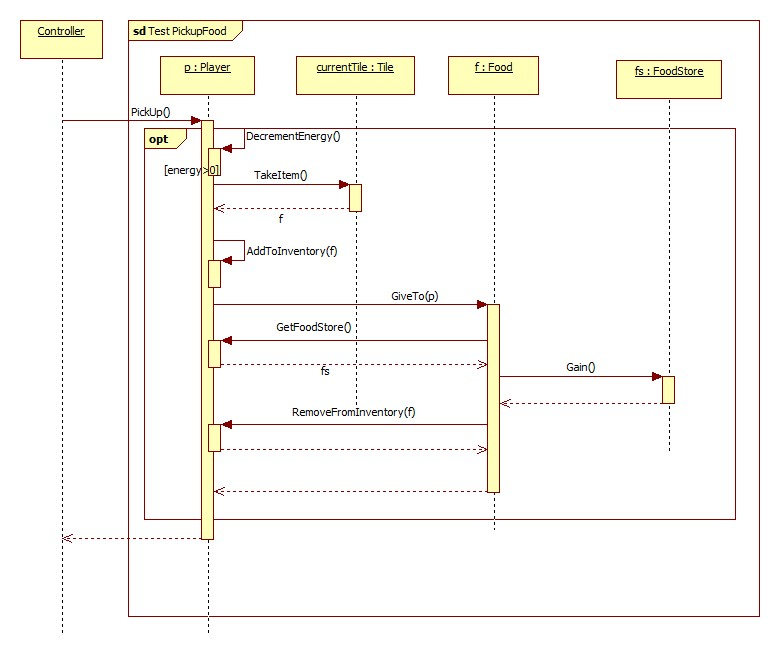
\includegraphics[width=17cm]{chapters/chapter05/diagrams/TestPickUpFood.jpg}
		\caption{Test PickUp Food}
		\label{fig:Test PickUp Food}
	\end{center}
\end{figure}

\begin{figure}[h]
	\begin{center}
		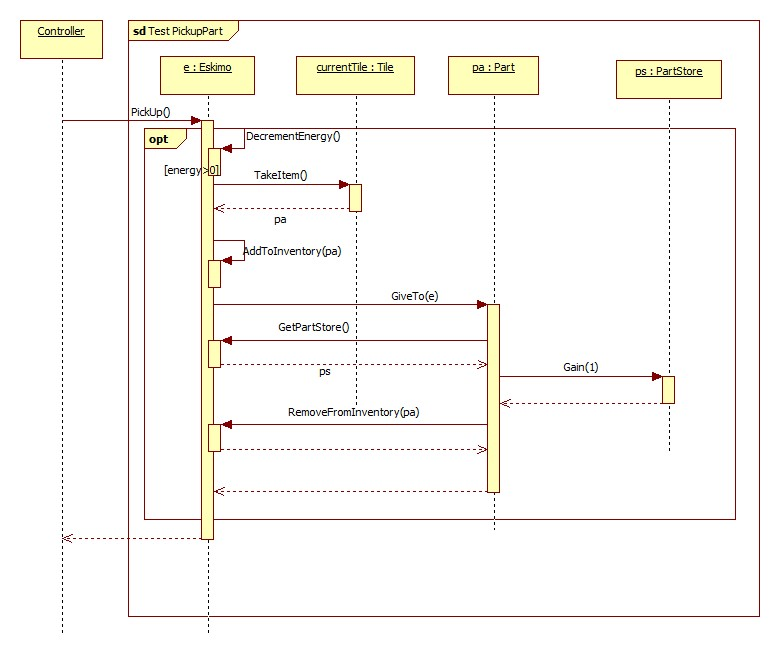
\includegraphics[width=17cm]{chapters/chapter05/diagrams/TestPickUpPart.jpg}
		\caption{Test PickUp Part}
		\label{fig:Test PickUp Part}
	\end{center}
\end{figure}

\begin{figure}[h]
	\begin{center}
		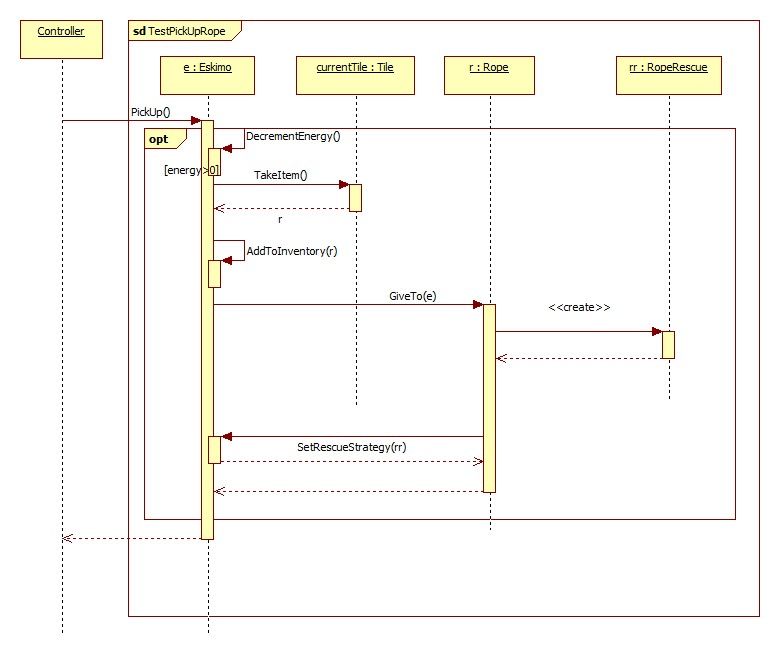
\includegraphics[width=17cm]{chapters/chapter05/diagrams/TestPickUpRope.jpg}
		\caption{Test PickUp Rope}
		\label{fig:Test PickUp Rope}
	\end{center}
\end{figure}

\begin{figure}[h]
	\begin{center}
		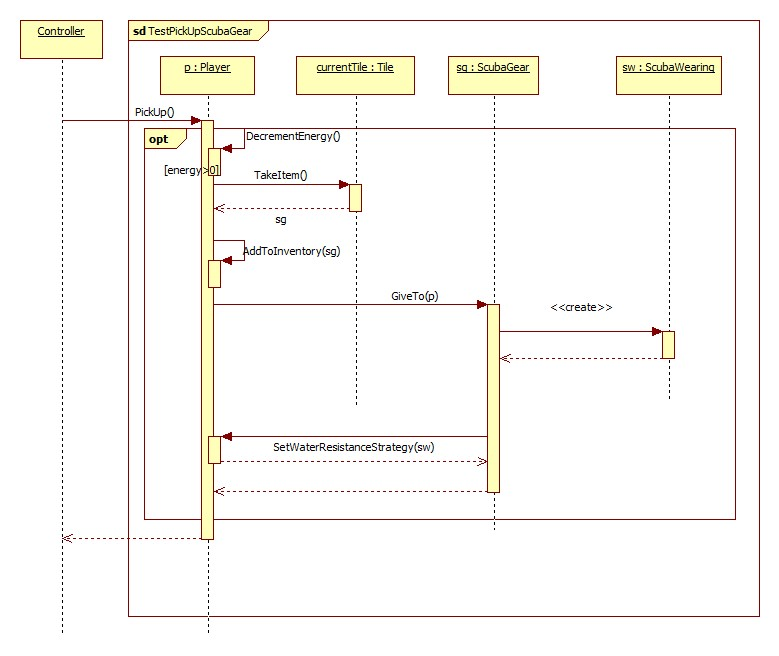
\includegraphics[width=17cm]{chapters/chapter05/diagrams/TestPickUpScubaGear.jpg}
		\caption{Test PickUp ScubaGear}
		\label{fig:Test PickUp ScubaGear}
	\end{center}
\end{figure}

\begin{figure}[h]
	\begin{center}
		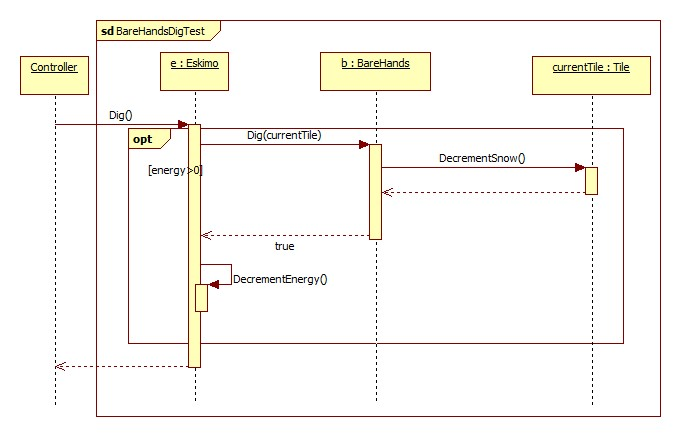
\includegraphics[width=17cm]{chapters/chapter05/diagrams/TestBareHandsDig.jpg}
		\caption{Test BareHandsDig}
		\label{fig:Test BareHandsDig}
	\end{center}
\end{figure}

\begin{figure}[h]
	\begin{center}
		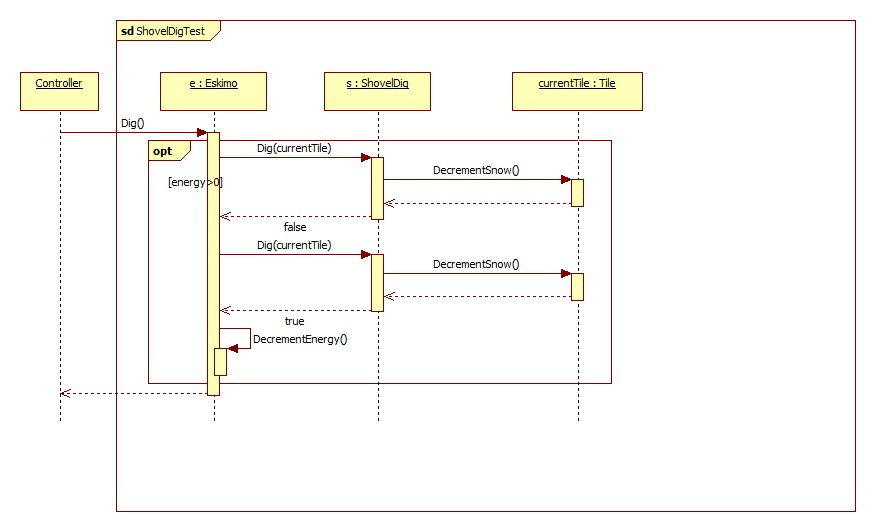
\includegraphics[width=17cm]{chapters/chapter05/diagrams/TestShovelDig.jpg}
		\caption{Test ShovelDig}
		\label{fig:Test ShovelDig}
	\end{center}
\end{figure}

\begin{figure}[h]
	\begin{center}
		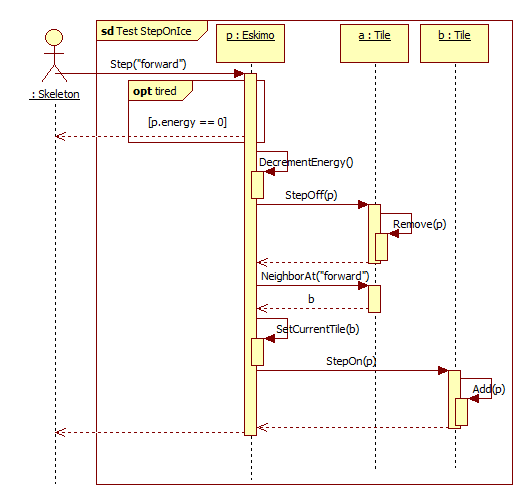
\includegraphics[width=17cm]{chapters/chapter05/diagrams/Test_StepOnIce.png}
		\caption{Test StepOnIce}
		\label{fig:Test StepOnIce}
	\end{center}
\end{figure}

\begin{figure}[h]
	\begin{center}
		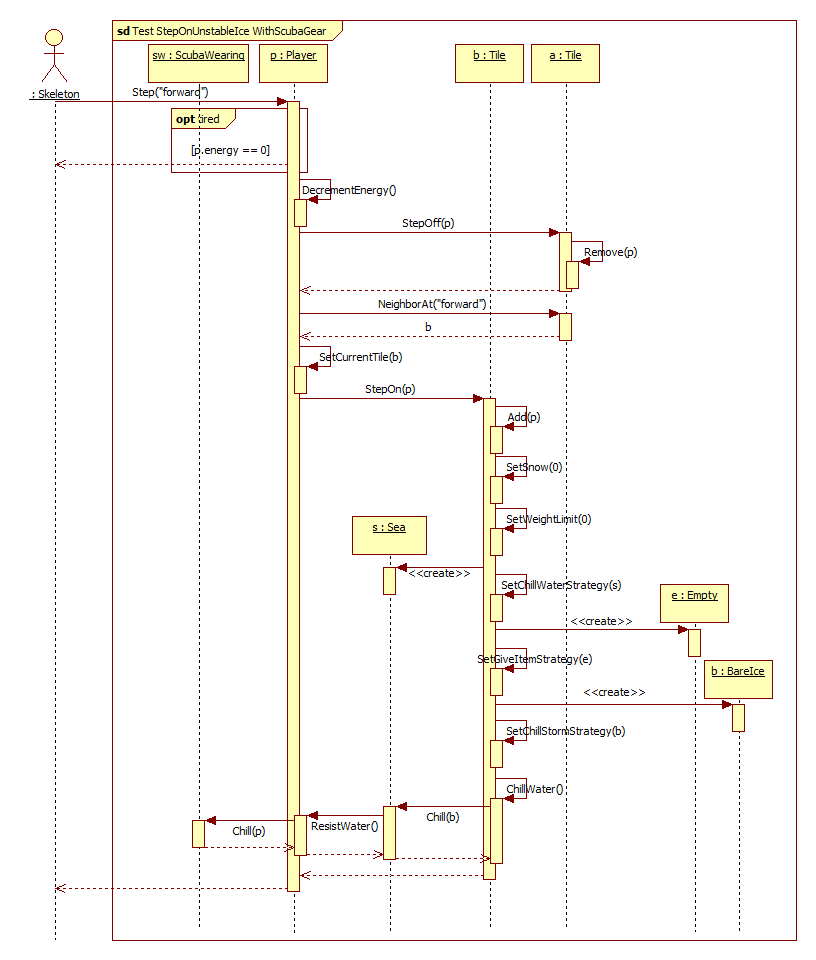
\includegraphics[width=17cm]{chapters/chapter05/diagrams/Test_StepOnUnstableIce_WithScubaGear.png}
		\caption{Test StepOnUnstableIce WithScubaGear}
		\label{fig:Test StepOnUnstableIce WithScubaGear}
	\end{center}
\end{figure}

\begin{figure}[h]
	\begin{center}
		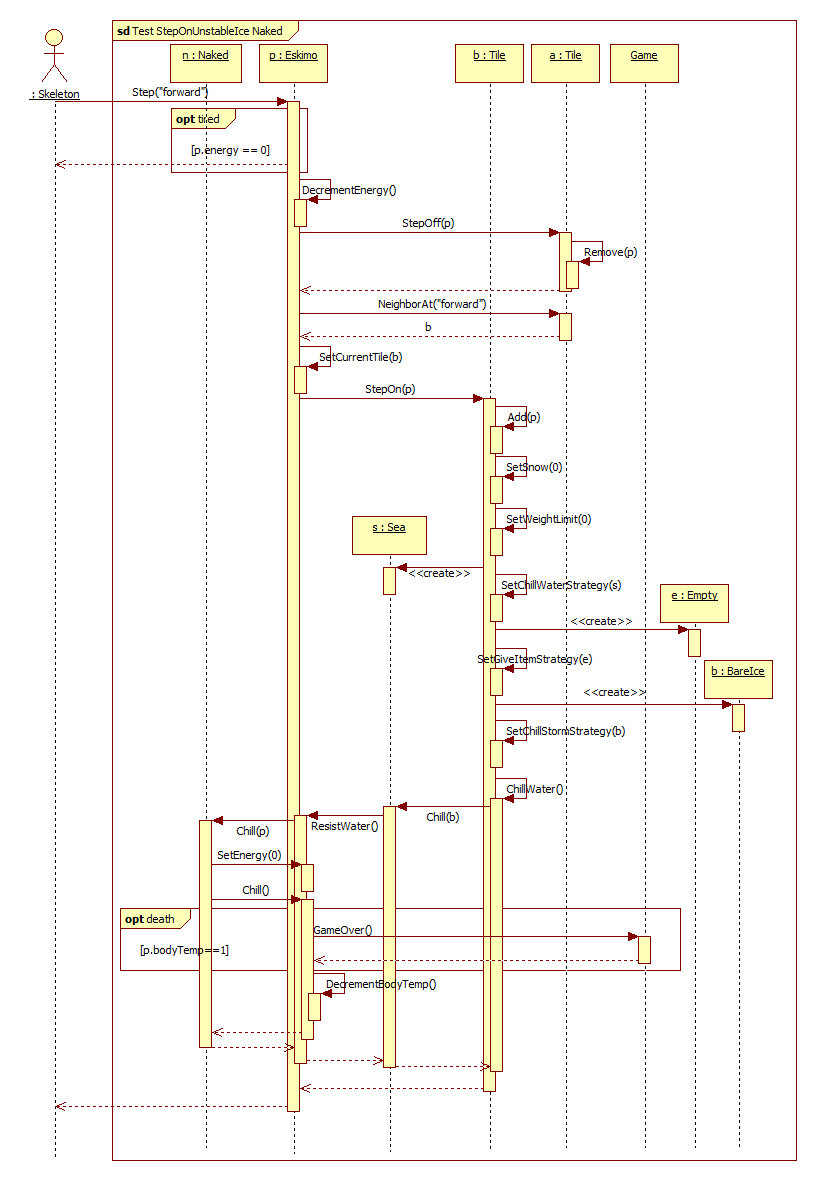
\includegraphics[width=17cm]{chapters/chapter05/diagrams/Test_StepOnUnstableIce_Naked.png}
		\caption{Test StepOnUnstableIce Naked}
		\label{fig:Test StepOnUnstableIce Naked}
	\end{center}
\end{figure}

\begin{figure}[h]
	\begin{center}
		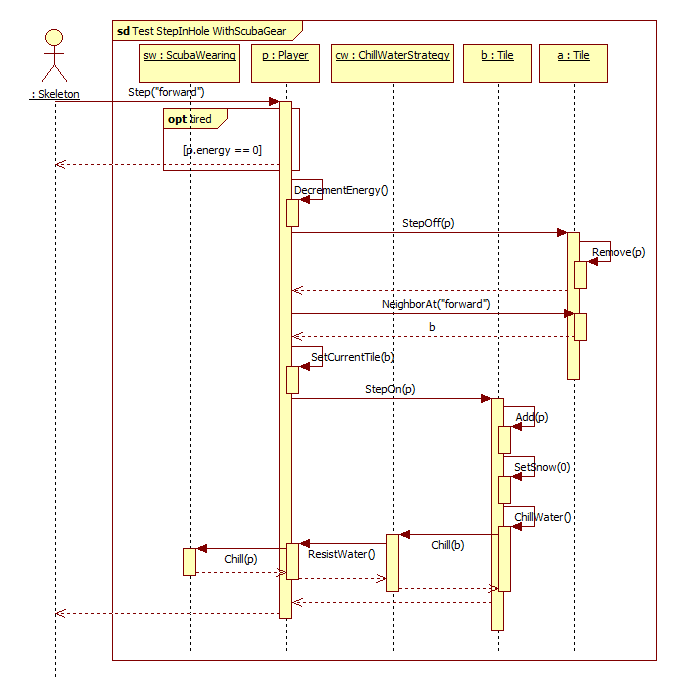
\includegraphics[width=17cm]{chapters/chapter05/diagrams/Test_StepInHole_WithScubaGear.png}
		\caption{Test StepInHole WithScubaGear}
		\label{fig:Test StepInHole WithScubaGear}
	\end{center}
\end{figure}

\begin{figure}[h]
	\begin{center}
		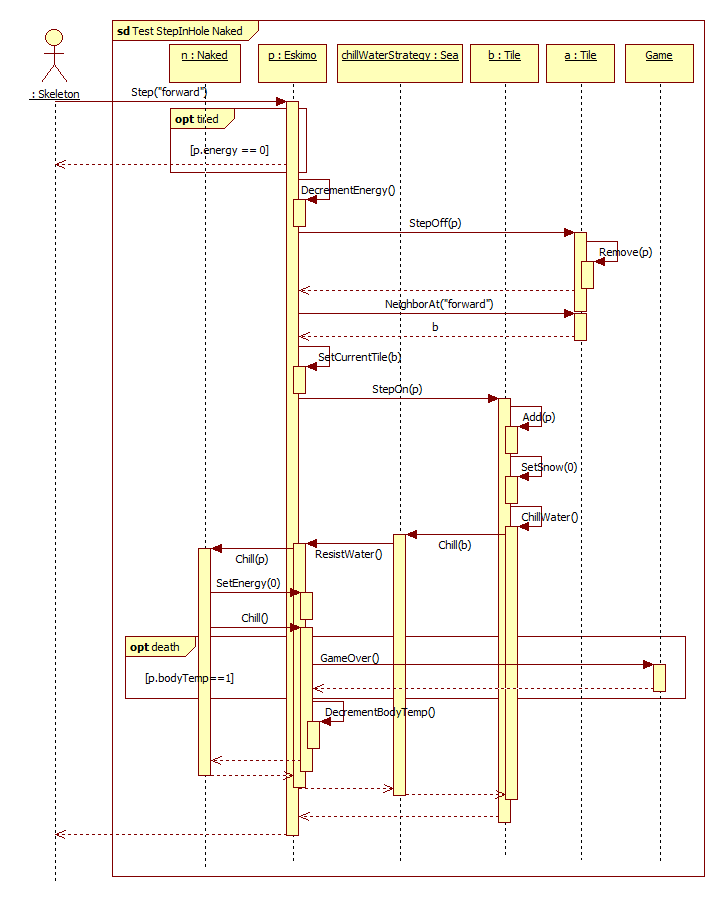
\includegraphics[width=17cm]{chapters/chapter05/diagrams/Test_StepInHole_Naked.png}
		\caption{Test StepInHole Naked}
		\label{fig:Test StepInHole Naked}
	\end{center}
\end{figure}

\begin{figure}[h]
	\begin{center}
		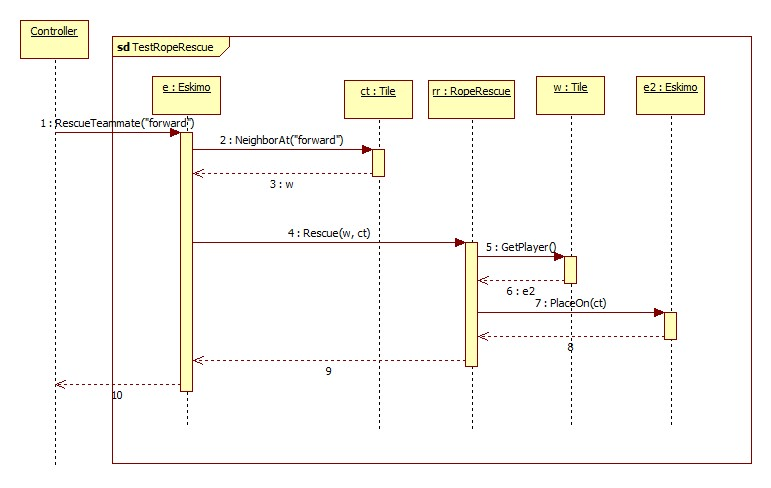
\includegraphics[width=17cm]{chapters/chapter05/diagrams/Test_RopeRescue.jpg}
		\caption{Test RopeRescue}
		\label{fig:Test RopeRescue}
	\end{center}
\end{figure}

\begin{figure}[h]
	\begin{center}
		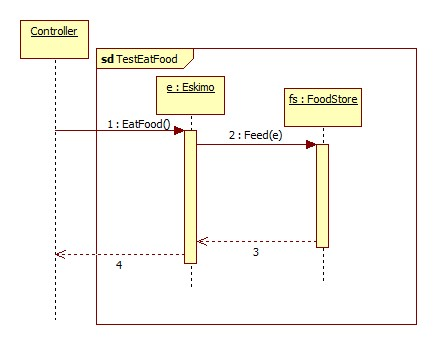
\includegraphics[width=17cm]{chapters/chapter05/diagrams/Test_EatFood.jpg}
		\caption{Test EatFood}
		\label{fig:Test EatFood}
	\end{center}
\end{figure}
\begin{figure}[h]
	\begin{center}
		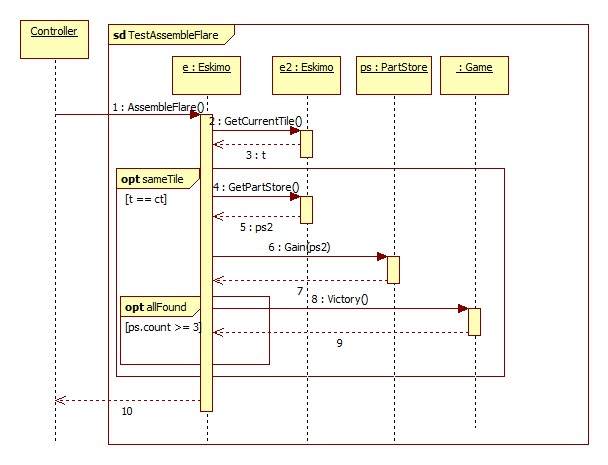
\includegraphics[width=17cm]{chapters/chapter05/diagrams/Test_AssembleFlare.jpg}
		\caption{Test AssembleFlare}
		\label{fig:Test AssembleFlare}
	\end{center}
\end{figure}

\begin{figure}[h]
	\begin{center}
		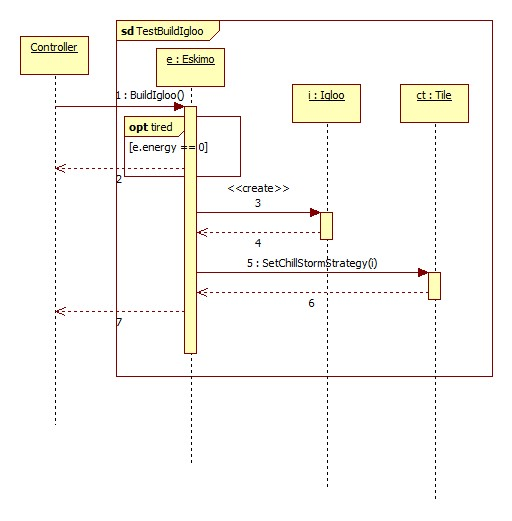
\includegraphics[width=17cm]{chapters/chapter05/diagrams/Test_BuildIgloo.jpg}
		\caption{Test BuildIgloo}
		\label{fig:Test BuildIgloo}
	\end{center}
\end{figure}

\begin{figure}[h]
	\begin{center}
		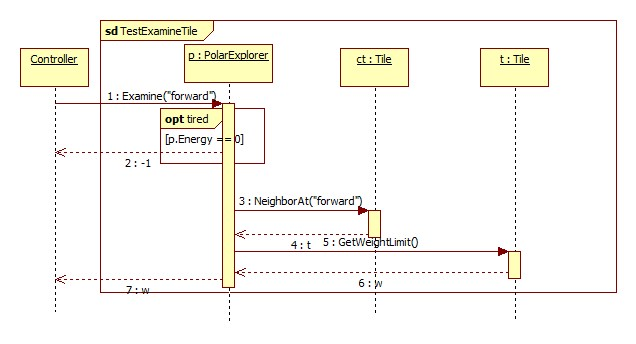
\includegraphics[width=17cm]{chapters/chapter05/diagrams/Test_ExamineTile.jpg}
		\caption{Test ExamineTile}
		\label{fig:Test ExamineTile}
	\end{center}
\end{figure}

\begin{figure}[h]
	\begin{center}
		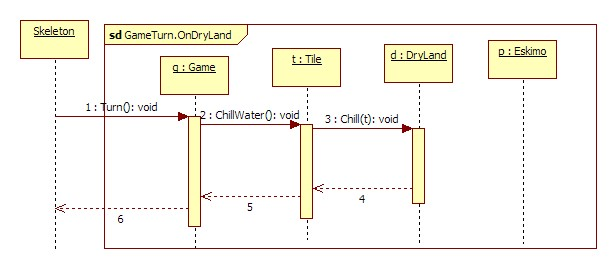
\includegraphics[width=17cm]{chapters/chapter05/diagrams/Test_Turn_OnStableIce.jpg}
		\caption{Test Turn OnStableIce}
		\label{fig:Test Turn OnStableIce}
	\end{center}
\end{figure}

\begin{figure}[h]
	\begin{center}
		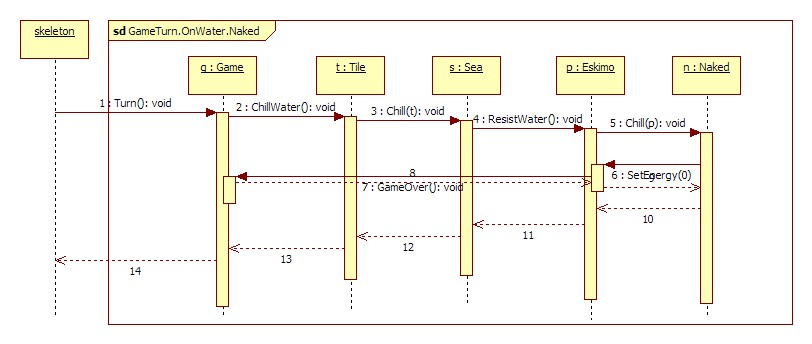
\includegraphics[width=17cm]{chapters/chapter05/diagrams/Test_Turn_InWater_Naked.jpg}
		\caption{Test Turn InWater Naked}
		\label{fig:Test Turn InWater Naked}
	\end{center}
\end{figure}

\begin{figure}[h]
	\begin{center}
		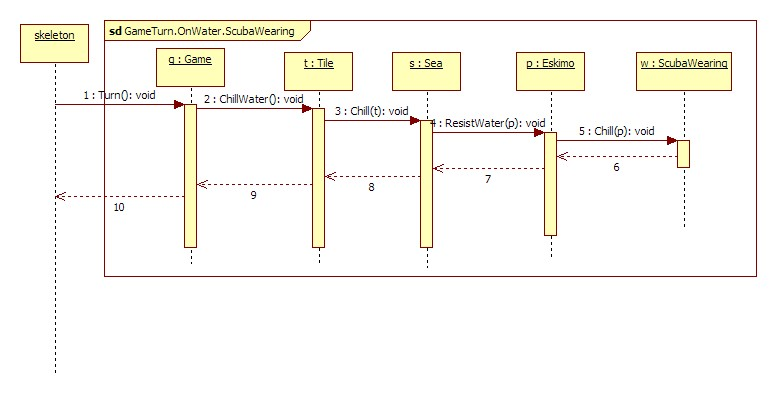
\includegraphics[width=17cm]{chapters/chapter05/diagrams/Test_Turn_InWater_WithScubaGear.jpg}
		\caption{Test Turn InWater WithScubaGear}
		\label{fig:Test Turn InWater WithScubaGear}
	\end{center}
\end{figure}

\begin{figure}[h]
	\begin{center}
		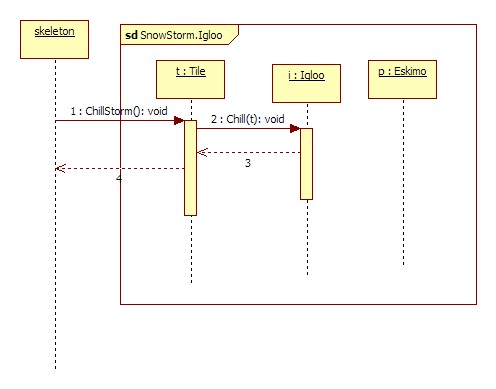
\includegraphics[width=17cm]{chapters/chapter05/diagrams/Test_ChillStorm_Igloo.jpg}
		\caption{Test ChillStorm Igloo}
		\label{fig:Test ChillStorm Igloo}
	\end{center}
\end{figure}

\begin{figure}[h]
	\begin{center}
		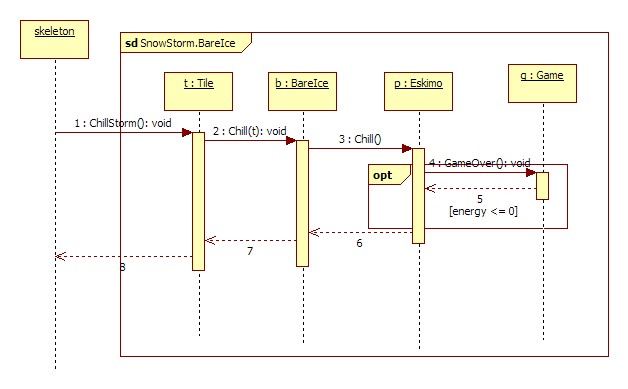
\includegraphics[width=17cm]{chapters/chapter05/diagrams/Test_ChillStorm_BareIce.jpg}
		\caption{Test ChillStorm BareIce}
		\label{fig:Test ChillStorm BareIce}
	\end{center}
\end{figure}



\pagebreak
\section{Kommunikációs diagramok}

\begin{figure}[h]
	\begin{center}
		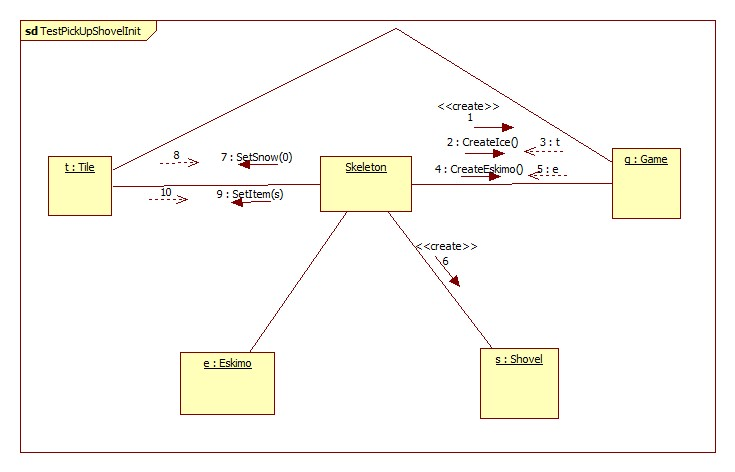
\includegraphics[width=17cm]{chapters/chapter05/diagrams/TestPickUpShovelInit.jpg}
		\caption{Test PickUp Shovel}
		\label{fig:Test PickUp Shovel}
	\end{center}
\end{figure}

\begin{figure}[h]
	\begin{center}
		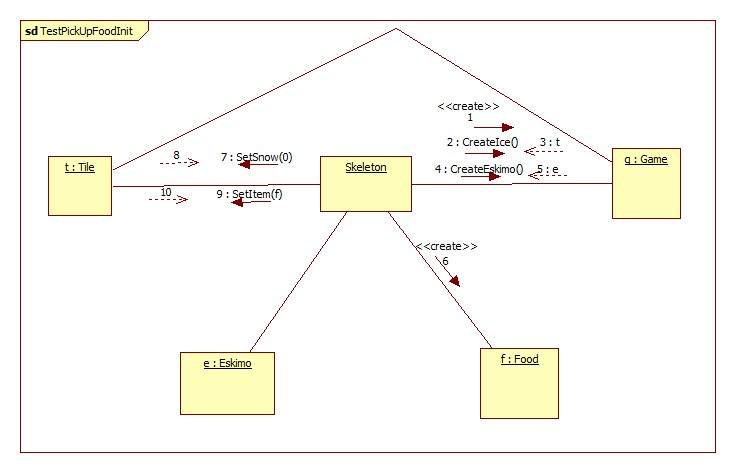
\includegraphics[width=17cm]{chapters/chapter05/diagrams/TestPickUpFoodInit.jpg}
		\caption{Test PickUp Food}
		\label{fig:Test PickUp Food}
	\end{center}
\end{figure}

\begin{figure}[h]
	\begin{center}
		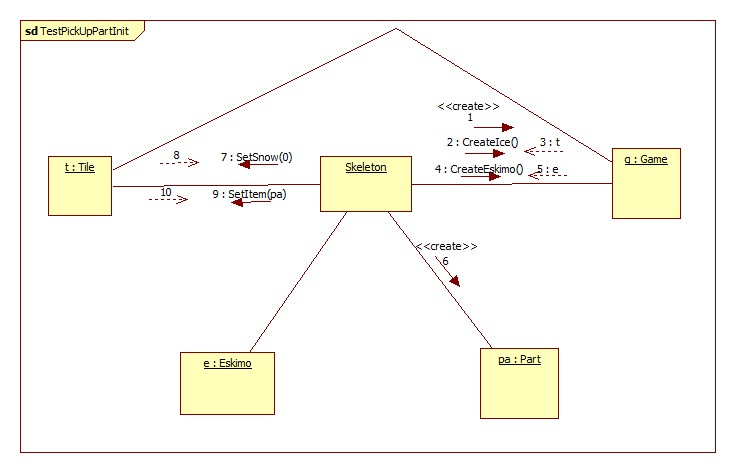
\includegraphics[width=17cm]{chapters/chapter05/diagrams/TestPickUpPartInit.jpg}
		\caption{Test PickUp Part}
		\label{fig:Test PickUp Part}
	\end{center}
\end{figure}

\begin{figure}[h]
	\begin{center}
		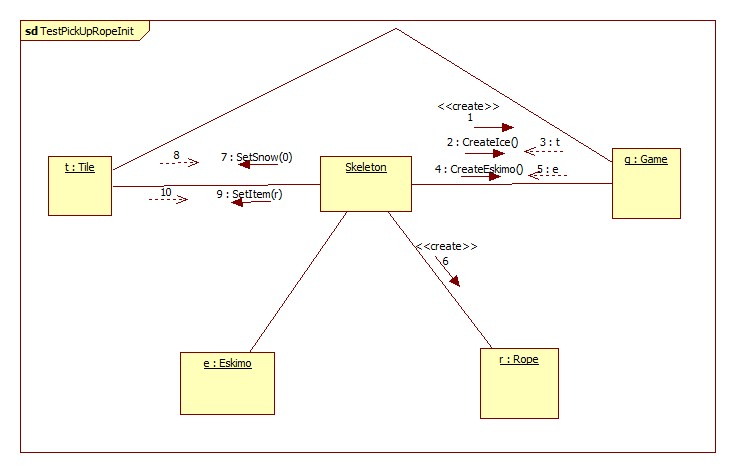
\includegraphics[width=17cm]{chapters/chapter05/diagrams/TestPickUpRopeInit.jpg}
		\caption{Test PickUp Rope}
		\label{fig:Test PickUp Rope}
	\end{center}
\end{figure}

\begin{figure}[h]
	\begin{center}
		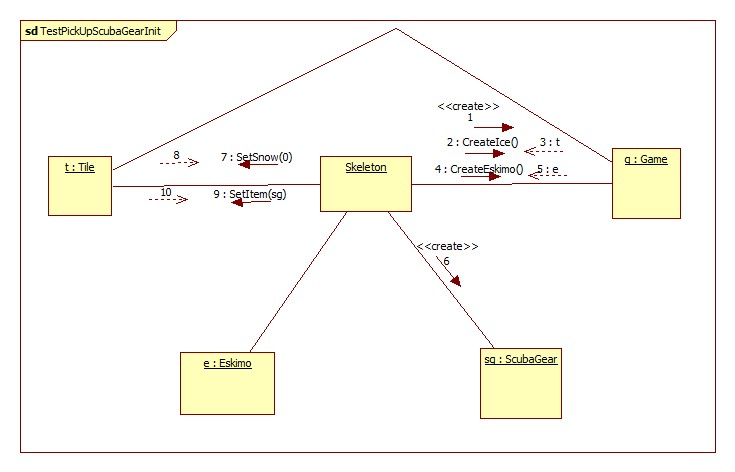
\includegraphics[width=17cm]{chapters/chapter05/diagrams/TestPickUpScubaGearInit.jpg}
		\caption{Test PickUp ScubaGear}
		\label{fig:Test PickUp ScubaGear}
	\end{center}
\end{figure}

\begin{figure}[h]
	\begin{center}
		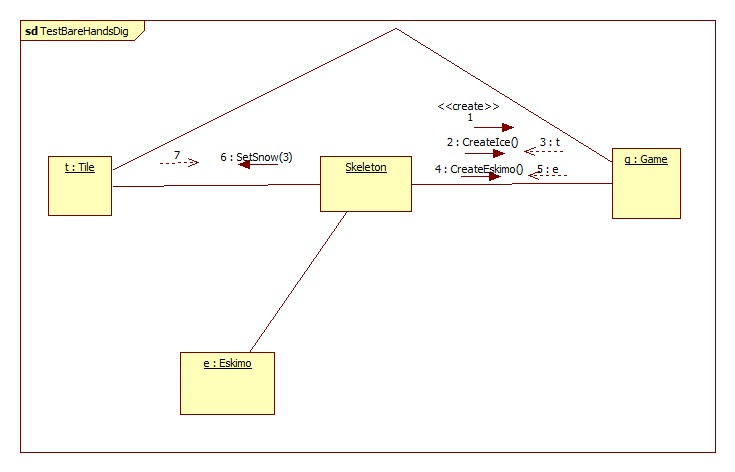
\includegraphics[width=17cm]{chapters/chapter05/diagrams/TestBareHandsDigInit.jpg}
		\caption{Test BareHandsDig}
		\label{fig:Test BareHandsDig}
	\end{center}
\end{figure}

\begin{figure}[h]
	\begin{center}
		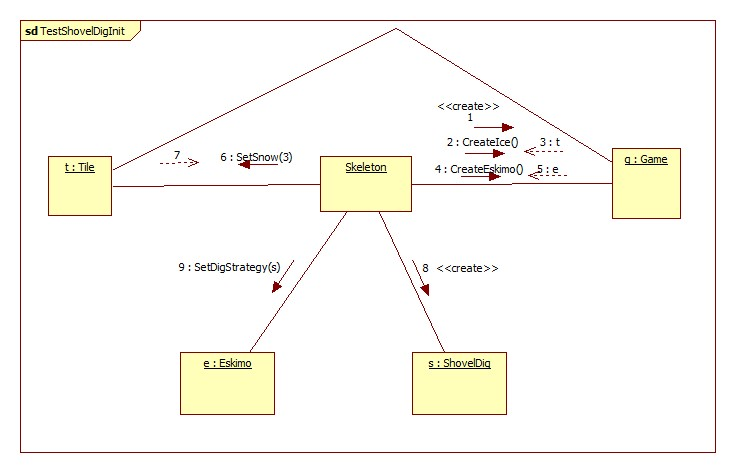
\includegraphics[width=17cm]{chapters/chapter05/diagrams/TestShovelDigInit.jpg}
		\caption{Test ShovelDig}
		\label{fig:Test ShovelDig}
	\end{center}
\end{figure}

\begin{figure}[h]
	\begin{center}
		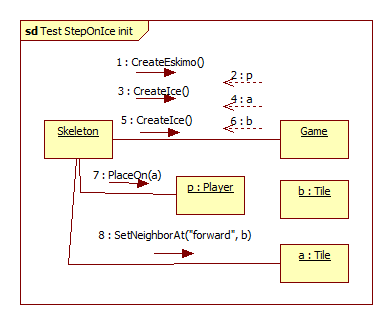
\includegraphics[width=17cm]{chapters/chapter05/diagrams/Test_StepOnIce_init.png}
		\caption{Test StepOnIce}
		\label{fig:Test StepOnIce}
	\end{center}
\end{figure}

\begin{figure}[h]
	\begin{center}
		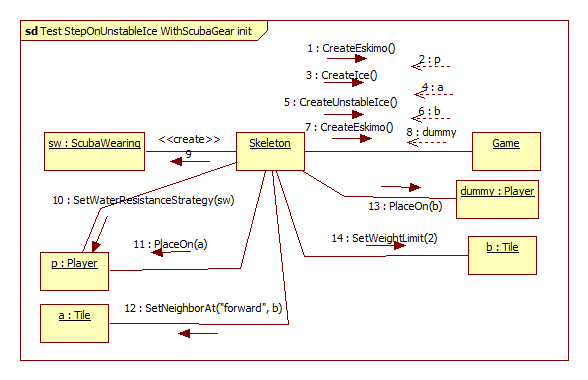
\includegraphics[width=17cm]{chapters/chapter05/diagrams/Test_StepOnUnstableIce_WithScubaGear_init.png}
		\caption{Test StepOnUnstableIce WithScubaGear}
		\label{fig:Test StepOnUnstableIce WithScubaGear}
	\end{center}
\end{figure}

\begin{figure}[h]
	\begin{center}
		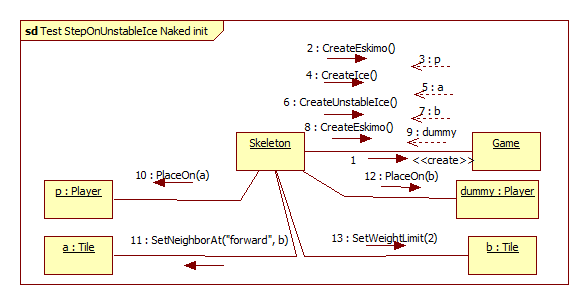
\includegraphics[width=17cm]{chapters/chapter05/diagrams/Test_StepOnUnstableIce_Naked_init.png}
		\caption{Test StepOnUnstableIce Naked}
		\label{fig:Test StepOnUnstableIce Naked}
	\end{center}
\end{figure}

\begin{figure}[h]
	\begin{center}
		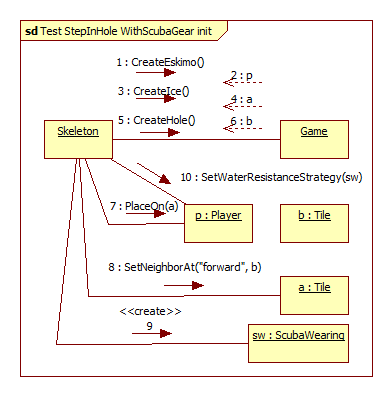
\includegraphics[width=17cm]{chapters/chapter05/diagrams/Test_StepInHole_WithScubaGear_init.png}
		\caption{Test StepInHole WithScubaGear}
		\label{fig:Test StepInHole WithScubaGear}
	\end{center}
\end{figure}

\begin{figure}[h]
	\begin{center}
		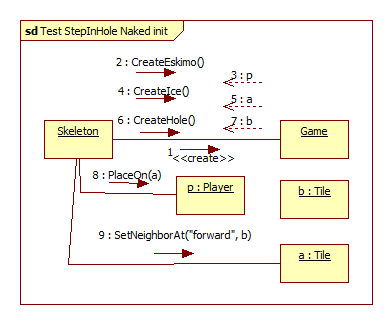
\includegraphics[width=17cm]{chapters/chapter05/diagrams/Test_StepInHole_Naked_init.png}
		\caption{Test StepInHole Naked}
		\label{fig:Test StepInHole Naked}
	\end{center}
\end{figure}

\begin{figure}[h]
	\begin{center}
		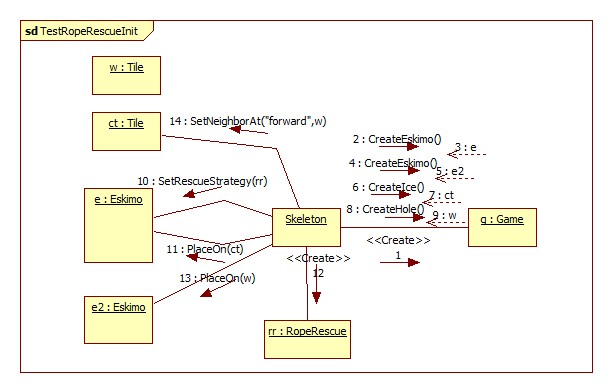
\includegraphics[width=17cm]{chapters/chapter05/diagrams/Test_RopeRescue_init.jpg}
		\caption{Test RopeRescue}
		\label{fig:Test RopeRescue}
	\end{center}
\end{figure}

\begin{figure}[h]
	\begin{center}
		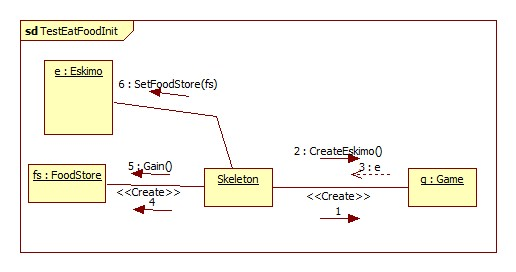
\includegraphics[width=17cm]{chapters/chapter05/diagrams/Test_EatFood_init.jpg}
		\caption{Test EatFood}
		\label{fig:Test EatFood}
	\end{center}
\end{figure}
\begin{figure}[h]
	\begin{center}
		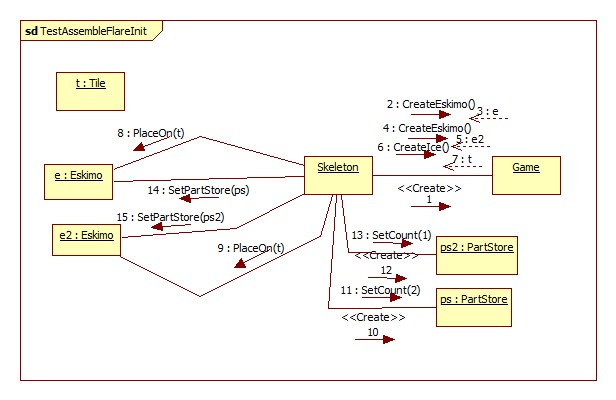
\includegraphics[width=17cm]{chapters/chapter05/diagrams/Test_AssembleFlare_init.jpg}
		\caption{Test AssembleFlare}
		\label{fig:Test AssembleFlare}
	\end{center}
\end{figure}

\begin{figure}[h]
	\begin{center}
		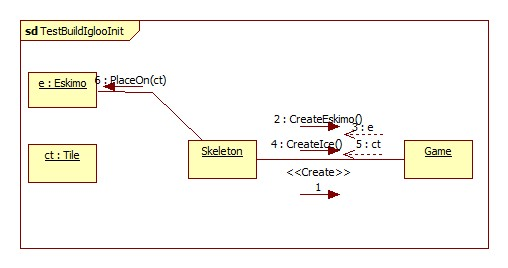
\includegraphics[width=17cm]{chapters/chapter05/diagrams/Test_BuildIgloo_init.jpg}
		\caption{Test BuildIgloo}
		\label{fig:Test BuildIgloo}
	\end{center}
\end{figure}

\begin{figure}[h]
	\begin{center}
		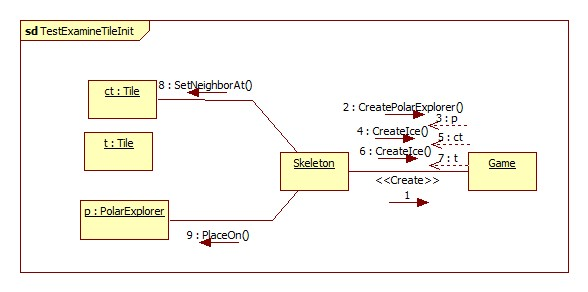
\includegraphics[width=17cm]{chapters/chapter05/diagrams/Test_ExamineTile_init.jpg}
		\caption{Test ExamineTile}
		\label{fig:Test ExamineTile}
	\end{center}
\end{figure}

\begin{figure}[h]
	\begin{center}
		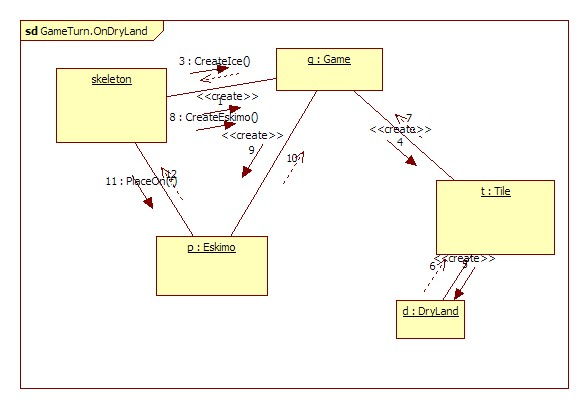
\includegraphics[width=17cm]{chapters/chapter05/diagrams/Test_Turn_OnStableIce_init.jpg}
		\caption{Test Turn OnStableIce}
		\label{fig:Test Turn OnStableIce}
	\end{center}
\end{figure}

\begin{figure}[h]
	\begin{center}
		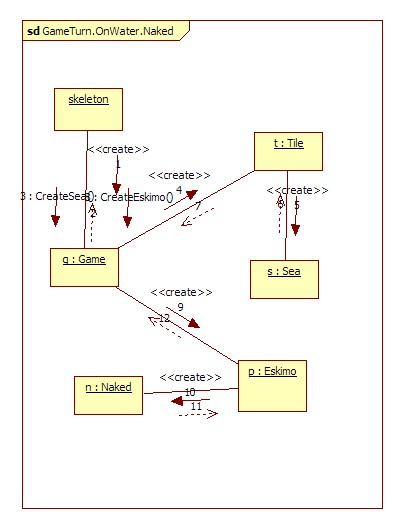
\includegraphics[width=17cm]{chapters/chapter05/diagrams/Test_Turn_InWater_Naked_init.jpg}
		\caption{Test Turn InWater Naked}
		\label{fig:Test Turn InWater Naked}
	\end{center}
\end{figure}

\begin{figure}[h]
	\begin{center}
		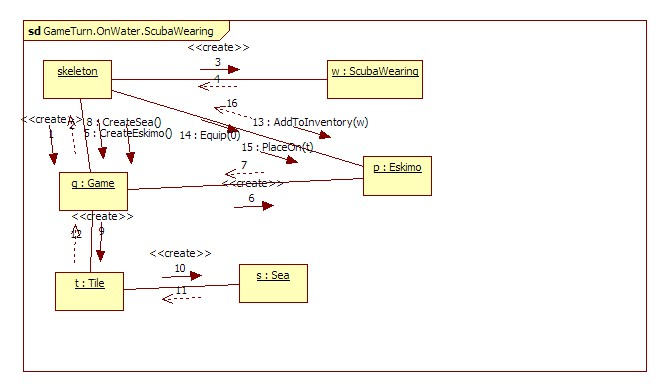
\includegraphics[width=17cm]{chapters/chapter05/diagrams/Test_Turn_InWater_WithScubaGear_init.jpg}
		\caption{Test Turn InWater WithScubaGear}
		\label{fig:Test Turn InWater WithScubaGear}
	\end{center}
\end{figure}

\begin{figure}[h]
	\begin{center}
		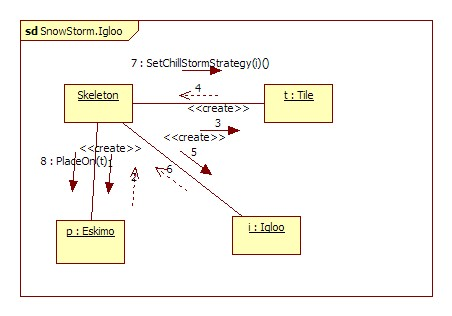
\includegraphics[width=17cm]{chapters/chapter05/diagrams/Test_ChillStorm_Igloo_init.jpg}
		\caption{Test ChillStorm Igloo}
		\label{fig:Test ChillStorm Igloo}
	\end{center}
\end{figure}

\begin{figure}[h]
	\begin{center}
		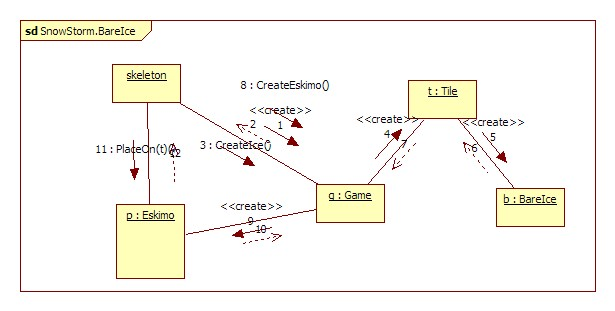
\includegraphics[width=17cm]{chapters/chapter05/diagrams/Test_ChillStorm_BareIce_init.jpg}
		\caption{Test ChillStorm BareIce}
		\label{fig:Test ChillStorm BareIce}
	\end{center}
\end{figure}
